\documentclass[12pt]{article}
\usepackage[utf8]{inputenc}
\usepackage{float}
\usepackage{amsmath}
\usepackage{tkz-graph}


\usepackage[hmargin=3cm,vmargin=6.0cm]{geometry}
%\topmargin=0cm
\topmargin=-2cm
\addtolength{\textheight}{6.5cm}
\addtolength{\textwidth}{2.0cm}
%\setlength{\leftmargin}{-5cm}
\setlength{\oddsidemargin}{0.0cm}
\setlength{\evensidemargin}{0.0cm}

%misc libraries goes here



\begin{document}

\section*{Student Information } 
%Write your full name and id number between the colon and newline
%Put one empty space character after colon and before newline
Full Name :  Aytaç SEKMEN \\
Id Number :  2575983 \\

% Write your answers below the section tags
\section*{Answer 1}
a)degree of b=3\\
degree of a=3\\
degree of c=3\\
degree of e=3\\
degree of d=2. So sum of degrees of all nodes is 14. Which is also twice of number of edges.\\\\
b) $\begin{bmatrix}
0& 1 & 1& 0& 1\\
1& 0 & 1& 0 &1\\
1& 1 & 0& 1 &0\\
0& 0 & 1& 0 &1\\
1& 1 & 0& 1 &0
\end{bmatrix}$\\\\ Since this is a adjacency matrix of graph G, there are 14 non-zero entries.\\\\
c)$Edge_1$ is between a and b vertices.\\
$Edge_2$ is between b and e vertices.\\
$Edge_3$ is between b and c vertices.\\
$Edge_4$ is between a and e vertices.\\
$Edge_5$ is between a and c vertices.\\
$Edge_6$ is between c and d vertices.\\
$Edge_7$ is between e and d vertices. And rows are edges(starting from $Edge_1$ and ending at $Edge_7$), columns are vertices(a,b,c,d,e).\\
$\begin{bmatrix}
1& 1 & 0& 0& 0\\
0& 1 & 0& 0 &1\\
1& 1 & 1& 0 &0\\
1& 0 & 0& 0 &1\\
1& 0 & 1& 0 &0\\
0& 0 & 1& 1 &0\\
0& 0 & 0& 1 &1
\end{bmatrix}$\\\\
So number of zero entries is actually 21.\\\\
d) Since a complete graph is a graph that has an edge between every single vertex in the graph. There is no complete subgraph of this graph with at least 4 vertices.\\\\e) We should check whether this graph is 2-colorable or not. For example if we color node-a with red we can colour b with blue, which is adjacent to a. But in this case we can't colour c with neither blue nor red. So this graph is not bipartite.
\\\\f) Since every edge can have 2 possible direction. There is actually $2^7=128$ possible directed graphs that have G as their underlying undirected graph.\\\\
g)Length of simple longest path is actually 4 (there is lots of path which has length 4 but one of them is this). a-b-c-d-e.\\\\
h)1. Because connected component of a graph G is maximal connected subgraph of G so connected component of graph G is itself. \\\\
i) By using theorem-1 given in the book for euler circuit. Since some of edges of G has degree 3 which is not even, the graph G has no euler circuit.\\\\
j) By using theorem-2 given in the book for euler circuit. ıf a graph doesn't have eule circuit then it must have exactly 2 vertices with odd degree, otherwise it has no euleriean path. Since graph G has 4 vertices with odd degree, there is actually no euler path in graph G.\\\\
k) Yes. a-b-e-d-c-a \\\\
l) Yes. a-c-b-e-d \\\\


\section*{Answer 2}
1) Graph G has 5 nodes. Graph-H has also 5 nodes.\\
2) Graph-G has 5 edges. Graph H has also 5 edges.\\
3) All nodes in graph-g has degree of 2. All graphs in graph-H has also degree of 2.\\4) Now we have to form 1-1 correspondence between these 2 graph. If I can form it, it means that they are isomorphic.\\\\
Step-1) Let's choose "a" as a starting point. Since they all have same degrees I can choose a' as a correspondent term to a.\\
Step-2) Let's take now b as adjacent node to a. And since all nodes have same degree I can choose e' or b' as a correspondence to b.\\
Step-3) Let's take now c as adjacent node to b. And I choose the c' as a correspondent node to c (no option left.).\\
Step-4) Let's take now d as adjacent node to c. And I choose the d' as a correspondent node to d (no option left.).\\
Step-5) Let's take now e as adjacent node to d. And I choose the e' as a correspondent node to e (no option left.).\\
Step-6) Let's form the adjacency matrix for these graphs.\\
Step-7) Adjaceny matrix for graph-G:\\\\
$\begin{bmatrix}
0& 1 & 0& 0& 1\\
1& 0 & 1& 0 &0\\
0& 1 & 0& 1 &0\\
0& 0 & 1& 0 &1\\
1& 0 & 0& 1 &0
\end{bmatrix}$\\\\
Step-8) Adjaceny matrix for graph-H:\\\\
$\begin{bmatrix}
0& 1 & 0& 0& 1\\
1& 0 & 1& 0 &0\\
0& 1 & 0& 1 &0\\
0& 0 & 1& 0 &1\\
1& 0 & 0& 1 &0
\end{bmatrix}$\\\\
Since these matrices are same, this means that Graph-G and graph-H are isomorphic.


\section*{Answer 3}
In this question, I have to go look for the shortest path to reach the adjacent vertices of each node while reaching at node-t from node-s.\\\\
1)Shortest path to reach the closest node from s is s-w which has length 3. So the closest vertex from vertex-s is w. Since I visited s and w, I add them to a set called visited and I will denote it by V=\{s,w\}.\\\\
2)Now I will look for the shortest path which starts from s and visit a vertex in set of visited and goes to the one which is not included in set of visited. (One of the alternative is s-v but it is not the shortest. So i dont choose it.) Path s-u has length=3 so this means that u is the second closest node to s. So now I add the vertex-u to the set of V=\{s,w,u\}\\\\
3)Now I will look for the shortest path which starts from s and visit a vertex in set of visited and goes to the one which is not included in set of visited. Even though path s-w-v has length 6, it is not the shortest path. Path s-v has length=5 so this means that v is the third closest vertex to s. So now I add the vertex-v to the set of V=\{s,w,u,v\}\\\\
4)Now I will look for the shortest path which starts from s and visit a vertex in set of visited and goes to the one which is not included in set of visited. Even though path s-w-x has length 11, it is not the shortest path. Path s-v-x has length=7 so this means that x is the fourth closest vertex to s. So now I add the vertex-x to the set of V=\{s,w,u,v,x\}\\\\
5)Now I will look for the shortest path which starts from s and visit a vertex in set of visited and goes to the one which is not included in set of visited. Even though path s-u-y has length 15, it is not the shortest path. Path s-v-x-y has length=8 so this means that y is the fifth closest vertex to s. So now I add the vertex-y to the set of V=\{s,w,u,v,x,y\}\\\\
6)Now I will look for the shortest path which starts from s and visit a vertex in set of visited and goes to the one which is not included in set of visited. Even though path s-w-z has length 15, it is not the shortest path. Path s-v-x-y-z has length=12 so this means that z is the sixth closest vertex to s. So now I add the vertex-z to the set of V=\{s,w,u,v,x,y,z\}\\\\
7)Now I will look for the shortest path which starts from s and visit a vertex in set of visited and goes to the one which is not included in set of visited. Even though path s-v-x-y-t has length 17, it is not the shortest path. Path s-v-x-y-z-t has length=15 so this means that t is the seventh closest vertex to s. So now I add the vertex-t to the set of V=\{s,w,u,v,x,y,z,t\}. So now I actually found the shortest path from s-t which is like s-v-x-y-z-t and has length 15.

\section*{Answer 4}
I will use Kruskal's Algorithm.\\\\
Step 1) For that I first choose the edge between d and k as a lowest weight.\\\\
Step 2) Secondly i continue with edges which have weight of 2. Since they dont form any circuit, I can add them. \{b, c\}, \{c, f\} and \{h-i\}.\\\\
Step 3) Since I added all edges which has weight 2. I will continue with edges which have weight 3. Since adding edges with weight 3 doesn't create any circuit as in the case of edges with weight 2, I can add all three edges which have weight 3.\\\\
Step 4) Now I should look at edges who have weight=4. I firstly will add the edge f-i. Because it doesn't create any circuit. Now I can add the edge \{e, f\}  and \{f, g\} because they also don't create any circuit. But since I add the \{f, g\} edge I can't add the \{g, j\} edge because it creates circuit.\\\\
Step 5) Since I have connected all the nodes, I actually found the minimum spanning tree.\\\\\\
a)\begin{table}[h!]
  \begin{center}
    \begin{tabular}{l|c|r} % <-- Alignments: 1st column left, 2nd middle and 3rd right, with vertical lines in between
      \textbf{Choice} & \textbf{Edge} & \textbf{weight}\\
      
      \hline
      1 & \{d,k\} & 2\\
      2 & \{b,c\} & 2\\
      3 & \{c,f\} & 2\\
      4 & \{h,i\} & 2\\
      5 & \{c,d\} & 3\\
      6 & \{a,b\} & 3\\
      7 & \{f,j\} & 3\\
      8 & \{f,g\} & 4\\
      9 & \{e,f\} & 4\\
      10& \{f,i\} & 4\\

    \end{tabular}
  \end{center}
\end{table}
 \\\\\\\\


b)
	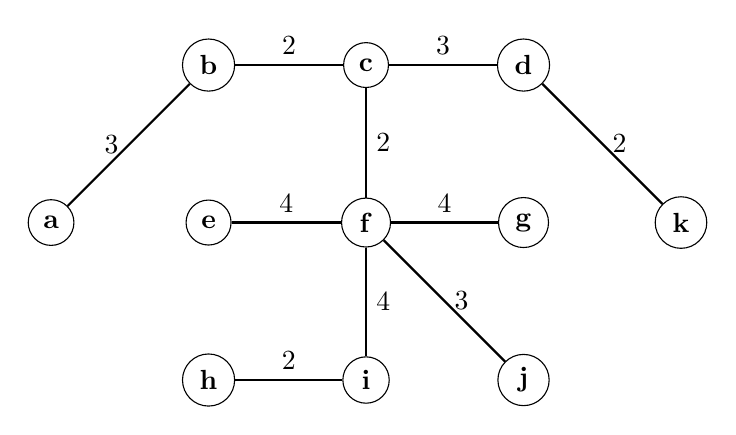
\begin{tikzpicture}
	
	\node[shape=circle,draw=black] (a) at (-2, 2)     {\textbf{a}};
	\node[shape=circle,draw=black] (b) at (0, 4)     {\textbf{b}};
	\node[shape=circle,draw=black] (c) at (2, 4)     {\textbf{c}};
	\node[shape=circle,draw=black] (d) at (4, 4)     {\textbf{d}};
	\node[shape=circle,draw=black] (e) at (0, 2)     {\textbf{e}};
	\node[shape=circle,draw=black] (f) at (2, 2)     {\textbf{f}};
	\node[shape=circle,draw=black] (g) at (4, 2)     {\textbf{g}};
	\node[shape=circle,draw=black] (h) at (0, 0)     {\textbf{h}};
	\node[shape=circle,draw=black] (i) at (2, 0)     {\textbf{i}};
	\node[shape=circle,draw=black] (j) at (4, 0)     {\textbf{j}};
	\node[shape=circle,draw=black] (k) at (6, 2)     {\textbf{k}};
	
	\path[-, thick] (a) edge node[left]{3} (b);
	

	\path[-, thick] (b) edge node[above]{2} (c);


	\path[-, thick] (c) edge node[above]{3} (d);
	\path[-, thick] (c) edge node[right]{2} (f);


	\path[-, thick] (d) edge node[right]{2} (k);
	\path[-, thick] (e) edge node[above]{4} (f);

	\path[-, thick] (f) edge node[above]{4} (g);

	\path[-, thick] (f) edge node[right]{4} (i);
	\path[-, thick] (f) edge node[right]{3} (j);

	\path[-, thick] (h) edge node[above]{2} (i);


	
	\end{tikzpicture}       So this is my spanning tree.\\\\



c) Actually this spanning tree is not unique because I can get different spanning tree if I've chosen the edge between node g and j instead of the edge between node f and g. Since they have the same weight this difference would do no change in terms of spanning term. 

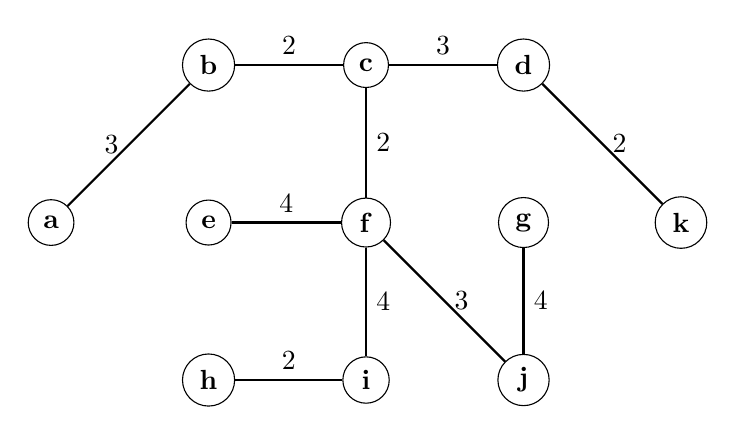
\begin{tikzpicture}
	
	\node[shape=circle,draw=black] (a) at (-2, 2)     {\textbf{a}};
	\node[shape=circle,draw=black] (b) at (0, 4)     {\textbf{b}};
	\node[shape=circle,draw=black] (c) at (2, 4)     {\textbf{c}};
	\node[shape=circle,draw=black] (d) at (4, 4)     {\textbf{d}};
	\node[shape=circle,draw=black] (e) at (0, 2)     {\textbf{e}};
	\node[shape=circle,draw=black] (f) at (2, 2)     {\textbf{f}};
	\node[shape=circle,draw=black] (g) at (4, 2)     {\textbf{g}};
	\node[shape=circle,draw=black] (h) at (0, 0)     {\textbf{h}};
	\node[shape=circle,draw=black] (i) at (2, 0)     {\textbf{i}};
	\node[shape=circle,draw=black] (j) at (4, 0)     {\textbf{j}};
	\node[shape=circle,draw=black] (k) at (6, 2)     {\textbf{k}};
	
	\path[-, thick] (a) edge node[left]{3} (b);
	

	\path[-, thick] (b) edge node[above]{2} (c);


	\path[-, thick] (c) edge node[above]{3} (d);
	\path[-, thick] (c) edge node[right]{2} (f);


	\path[-, thick] (d) edge node[right]{2} (k);
	\path[-, thick] (e) edge node[above]{4} (f);

	\path[-, thick] (g) edge node[right]{4} (j);

	\path[-, thick] (f) edge node[right]{4} (i);
	\path[-, thick] (f) edge node[right]{3} (j);

	\path[-, thick] (h) edge node[above]{2} (i);


	
	\end{tikzpicture}       For example this is an another spanning tree.\\\\
\end{document}